\chapter{Implementation}

In this chapter a reinforcement learning algorithm based on TD3 will be implemented that will be the framework for the reward function analysis in chapter 4.

\section{Environment and Interface}
Environment erklären - schnittstelle mit openAI gym - observation und action state erklären - einbau von algorithmus mit bild schnittstelle algorithmus zu environment 

\section{Algorithm Implementation}
TD3 is an off policy actor-critic algorithm based on the deep deterministic policy gradient algorithm \cite{lillicrap2015continuous}, with the enhancements of using Double Q-learning for the critics, delayed policy updates and target policy smoothing \cite{fujimoto2018}.
Actor-critic learning is a reinforcement-learning method that simultaneously learns a policy function and a value function. It is a combination of policy learning and Q-learning. The actor learns the policy function, which decides what actions to take, and critic learns the value function, by using Q-learning, which helps to improve the policy function.
Figure \ref{fig:TD3_graph} shows TD3 graphically while \ref{fig:TD3_pseudo} shows the rough structure of the algorithm using pseudo code. The code for the implementation of the algorithm this thesis is implemented in Python using Tensorflow 2 with the Keras API.

\begin{figure} 
	\centering
	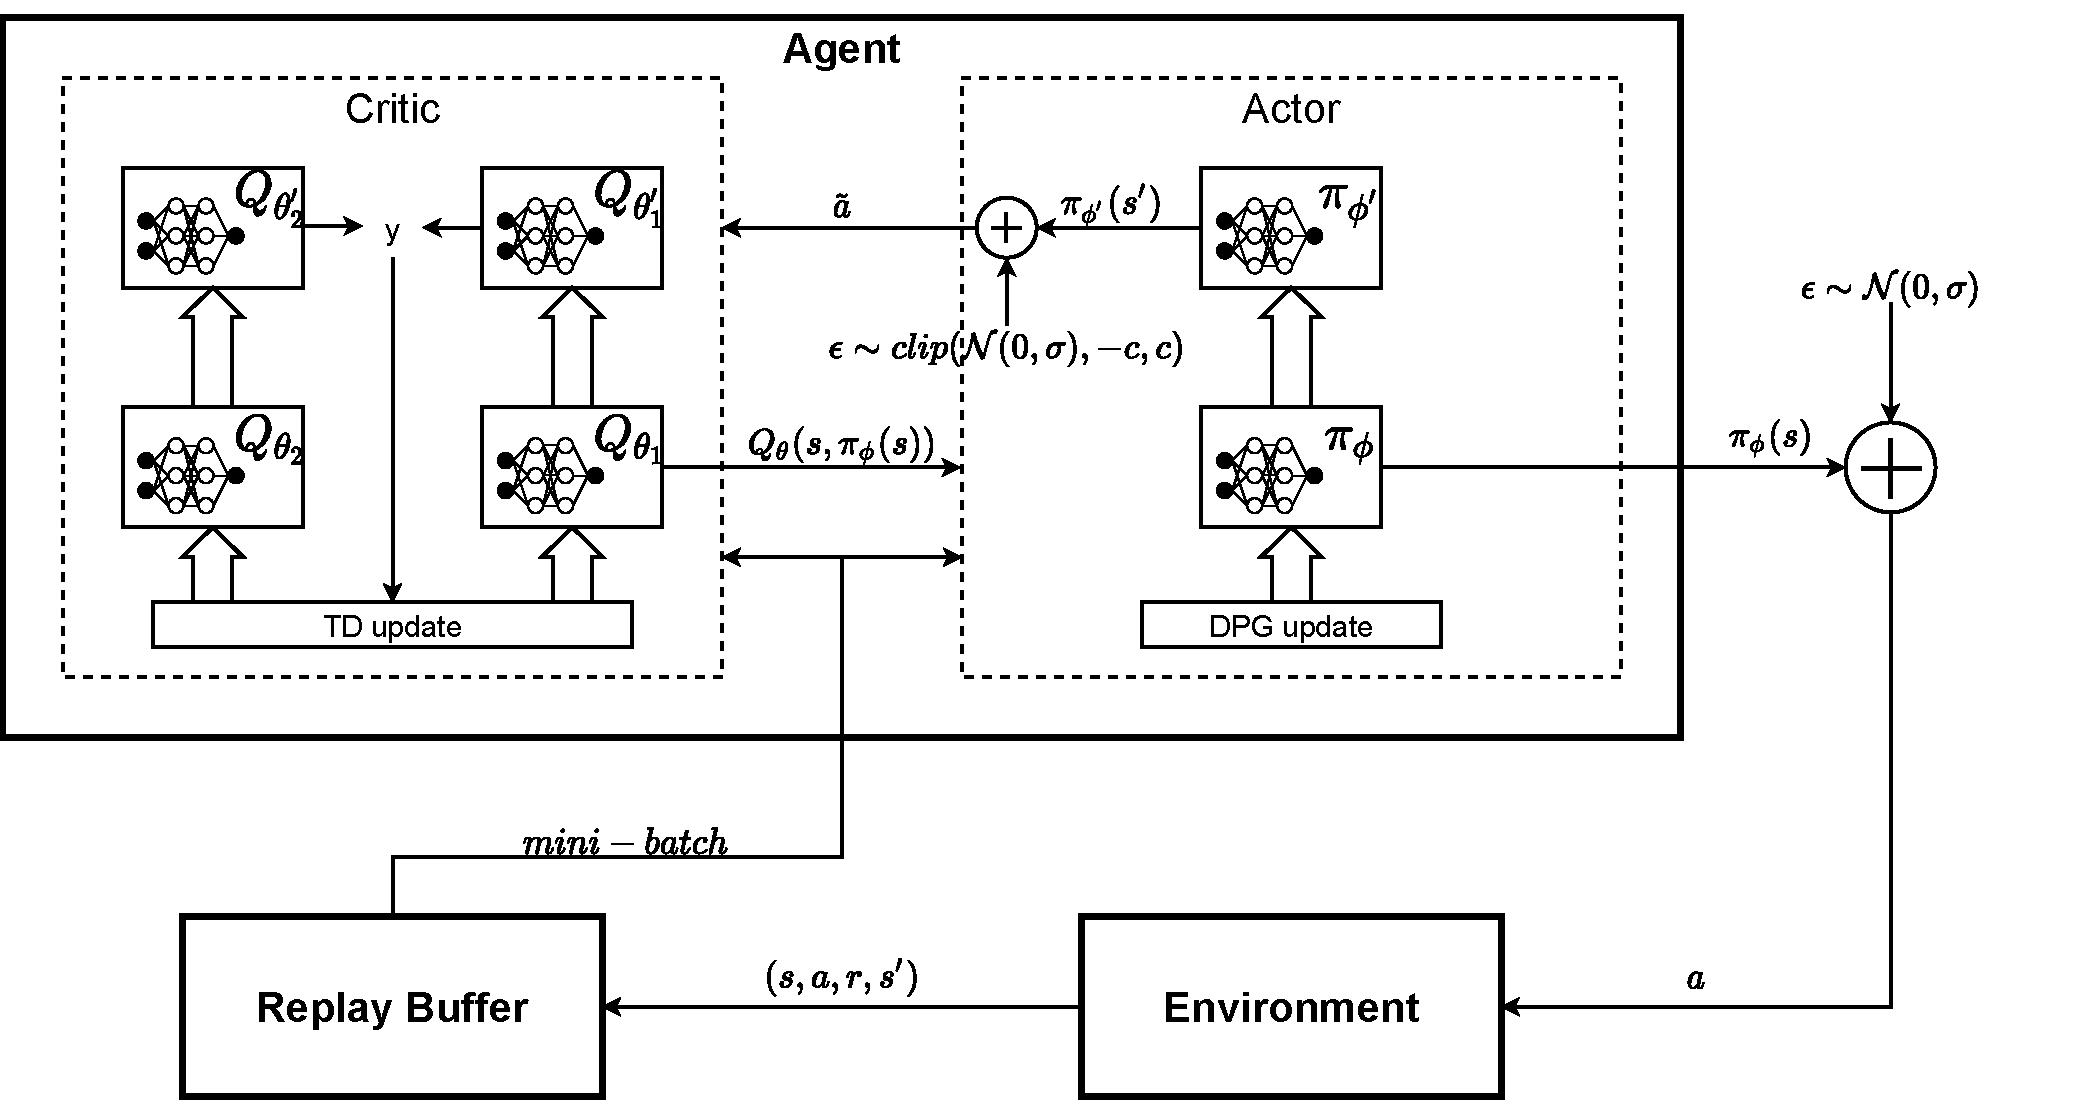
\includegraphics[scale=0.38]{img/Logo/TD3_graph.pdf}
	\caption{Graph of TD3}
	\label{fig:TD3_graph}
\end{figure}

\begin{figure} 
	\centering
	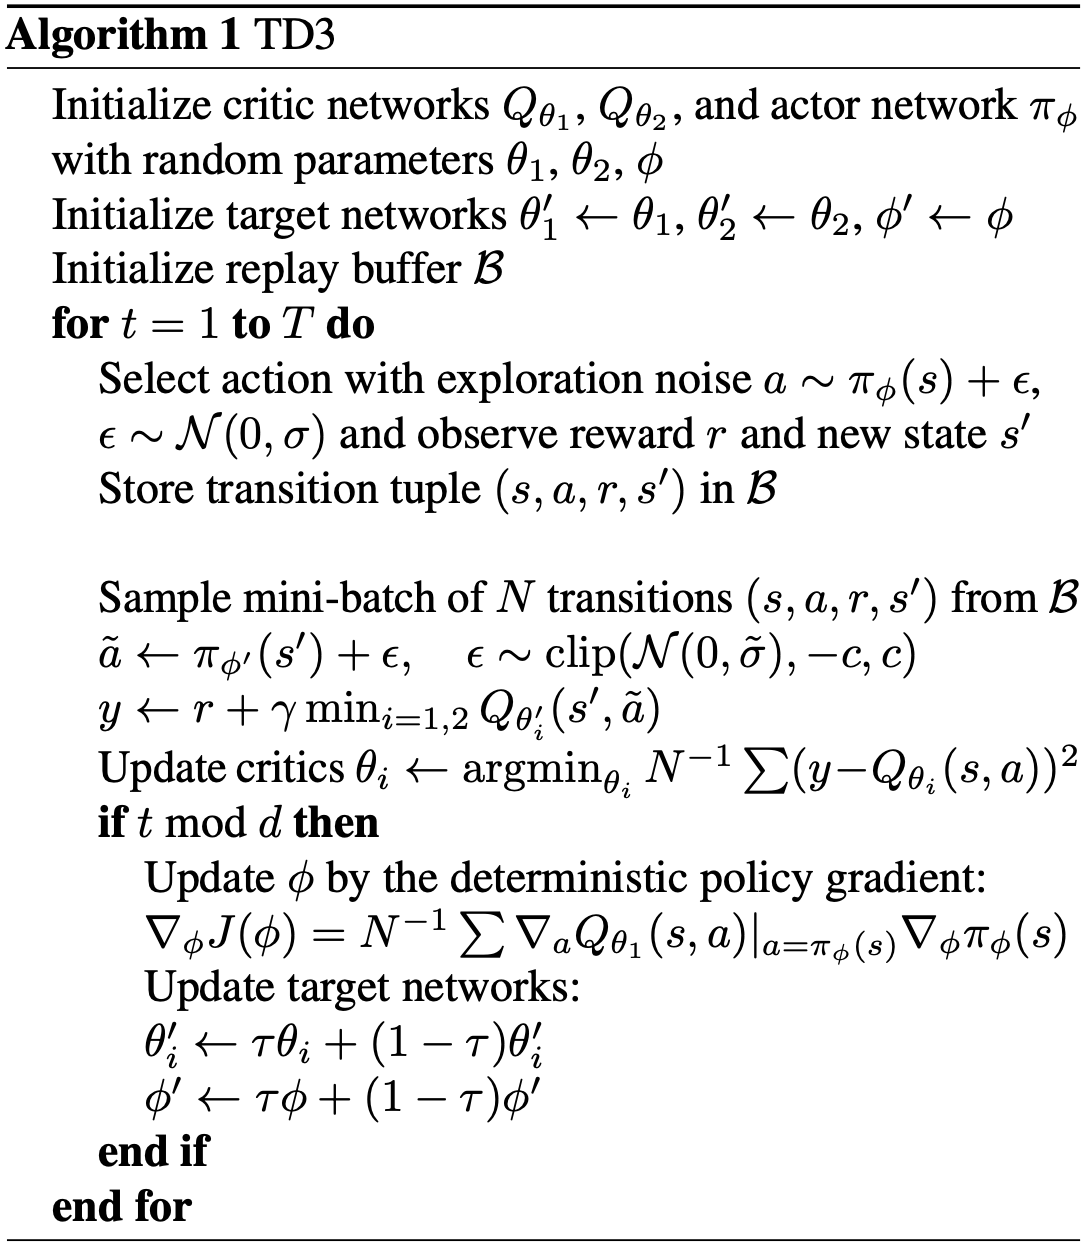
\includegraphics[scale=0.5]{img/Logo/TD3_pseudocode.png}
	\caption{TD3 pseudo code}
	\label{fig:TD3_pseudo}
\end{figure}

\subsection{Actor and Critic}
As shown in \ref{fig:TD3_pseudo} the first steps of the algorithm are to initialize the critic and the actor. Therefore artificial neural networks are used.
\newline \newline
\textbf{Artificial Neural Networks:}
In figure \ref{fig:NNConstruction} a general construction of an Artificial Neural Network (ANN) is illustrated.

\begin{figure} 
	\centering
	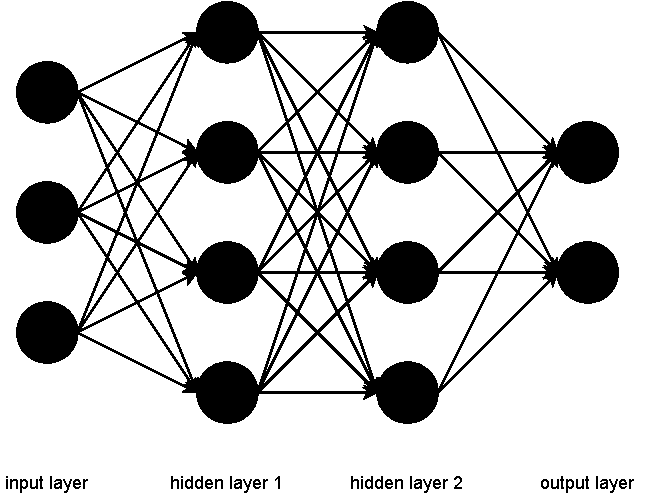
\includegraphics[scale=0.8]{img/Logo/NNConstruction.pdf}
	\caption{Artificial Neural Network}
	\label{fig:NNConstruction}
\end{figure}

\begin{figure} 
	\centering
	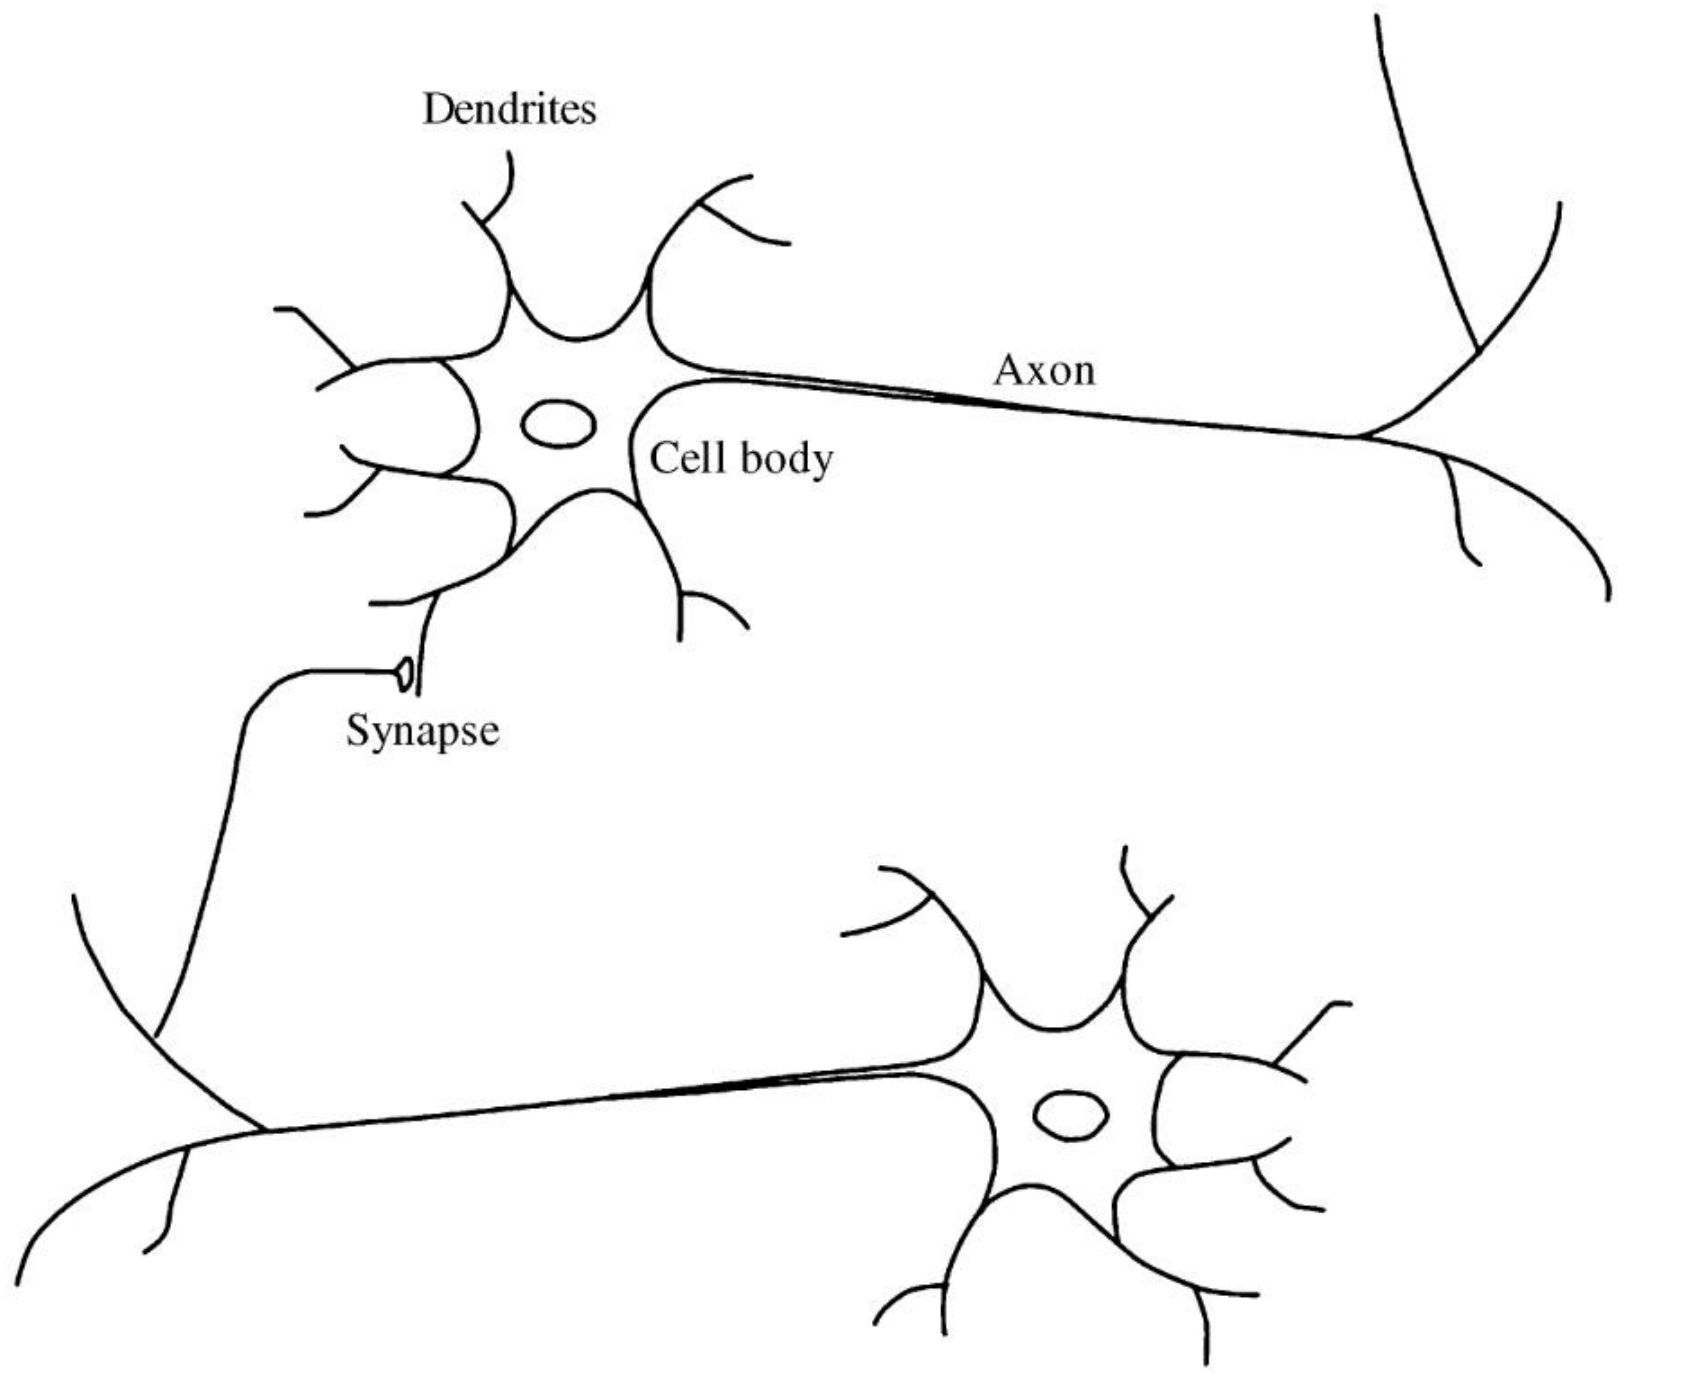
\includegraphics[scale=0.2]{img/Logo/neurons.png}
	\caption{Model of biological Neurons}
	\label{fig:neurons}
\end{figure}

An ANN basically consists of an input layer, which contains inputs with real numbered values, hidden layers and one output layer. The number of artificial neurons in a layer is not predetermined and so is the number of hidden layers. The artificial neurons of the layers can be linked to artificial neurons of other layers in any constellation. Depending on the way the artificial neurons are connected, there are numerous different types of ANNs. The type needed for this implementation is the feed forward network, which is characterized by the fact, that artificial neurons of a layer are only linked to artificial neurons of the following layer or layers. \cite{schmidhuber2015deep} \cite{shanmuganathan2016artificial}
The role model for ANNs comes from the human brain, that consists of about $10^{11}$ neurons with about $10^4$ connections each. Figure \ref{fig:neurons} shows a simplified diagram of two biological neurons. The dendrites carry electrical signals into the cell body. The cell body sums and thresholds these signals and the axon carries the signal to other neurons. The synapse is the point of contact of an axon and a dendrite of another neuron.\cite{CI} 

Based on McCulloch's and Pitts' mathematical model of a neuron \cite{pitts1947we}, Rosenblatt introduced an artificial neuron model called the perceptron \cite{rosenblatt1958perceptron} shown in figure \ref{fig:perceptron}.

\begin{figure} 
	\centering
	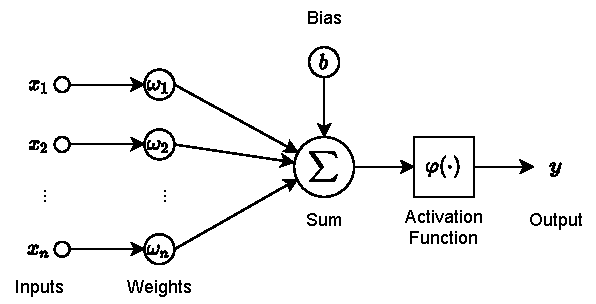
\includegraphics[scale=0.6]{img/Logo/perceptron.pdf}
	\caption{Perceptron}
	\label{fig:perceptron}
\end{figure}

The concept of the artificial neuron is divided in the following steps: \newline
\textbf{Inputs:} \newline
The inputs can either be a signal coming from a certain system, or be the output of a previous neuron. This depends on the location of the neuron being either inside the input layer or not. \newline
\textbf{Weights:} \newline
Every input is weighted with a certain value, which specifies the influence of the input to this neuron. The weights can be adjusted by a machine learning algorithm in order to reach a desired behaviour of the network. \newline
\textbf{Bias:} \newline
The bias value shifts the input net and can similarly to the weights be adjusted by a machine learning algorithm. \newline
\textbf{Sum and Activation Function:} \newline
The bias and the inputs multiplied by their weights get summed up, as shown in equation\ref{sum}. The activation function calculates the final output value of the perceptron using the summed up value as shown in equation \ref{activation}.  \newline

\begin{equation}
	sum = b + \sum_{i = 1}^n x_i \omega_i
	\label{sum}
\end{equation}

\begin{equation}
	y = \varphi(sum)
	\label{activation}
\end{equation}

There are a lot of different activation functions. In this implementation only the Rectifier Linear Unit (ReLU) function \ref{fig:relu} and the hyperbolic tangent (tanh) function \ref{fig:tanh} are used.

\begin{figure} 
	\centering
	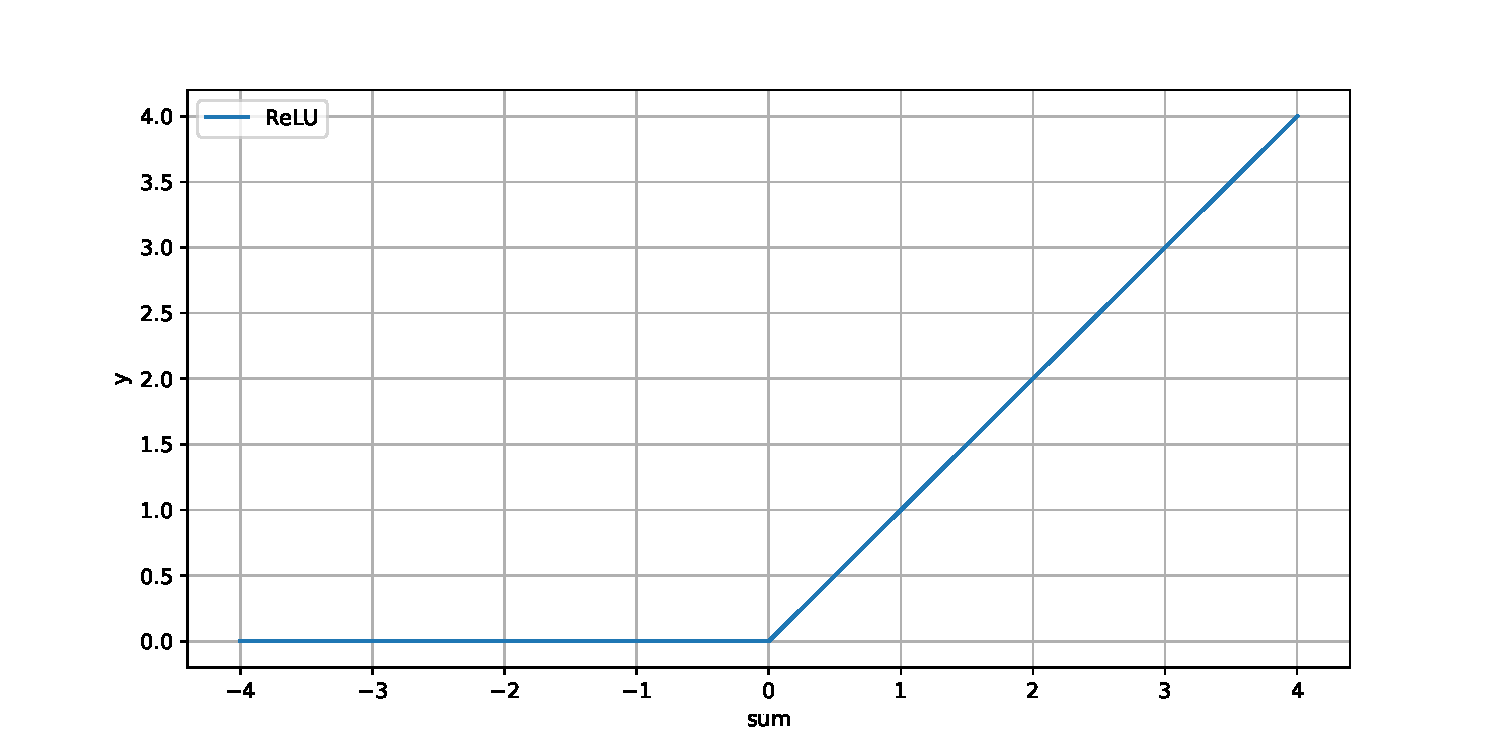
\includegraphics[scale=0.2]{img/Logo/relu.pdf}
	\caption{ReLU}
	\label{fig:relu}
\end{figure}

\begin{figure} 
	\centering
	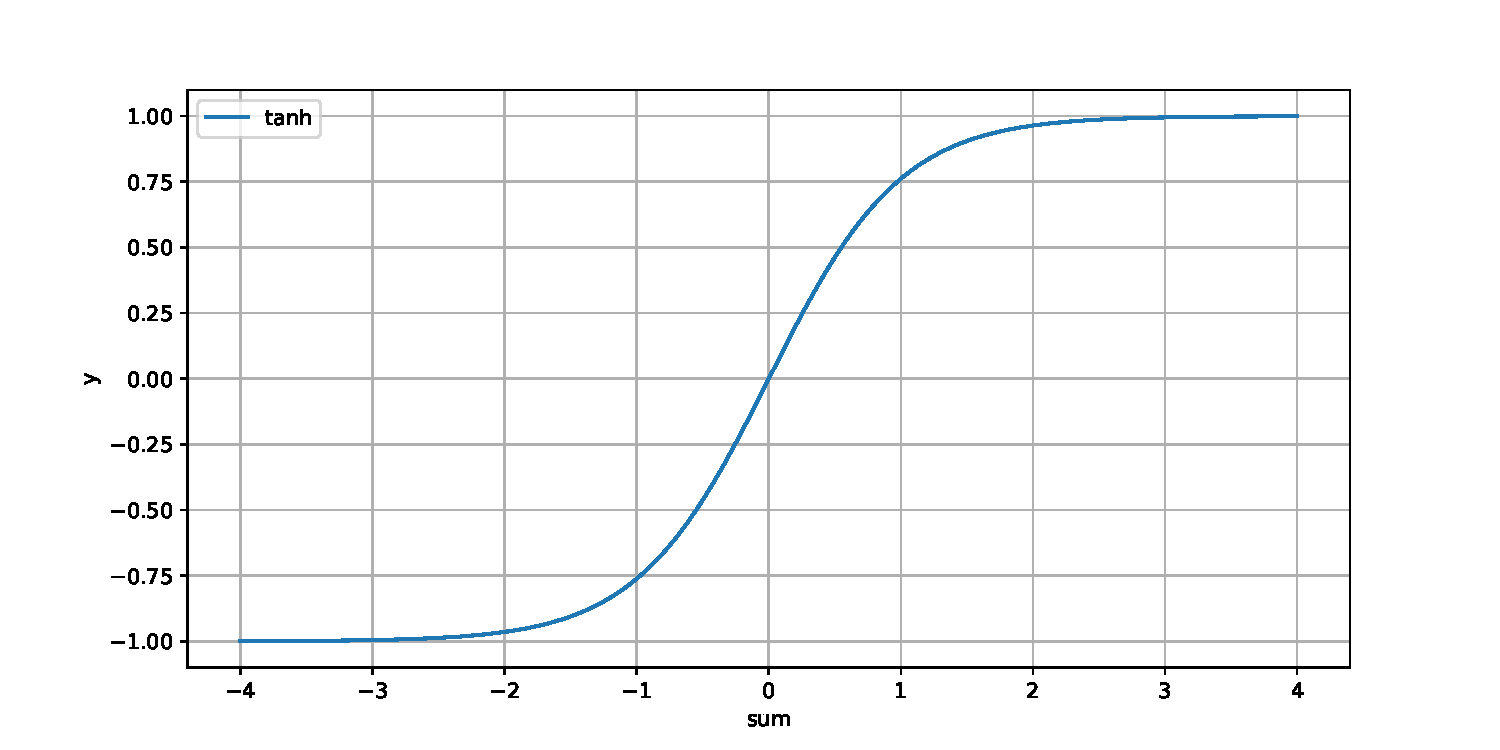
\includegraphics[scale=0.2]{img/Logo/tanh.pdf}
	\caption{tanh}
	\label{fig:tanh}
\end{figure}

\subsection{Deep Q-Learning}
\subsection{Policy Gradient}

\subsection{Build Agent}
jo
\subsubsection{Actor and Critic}
actor critic networks and target networks with mathematical equations
and number of layers, nodes... 
\subsubsection{Replay Buffer and Gaussian Noise}
input layer states and actions, output layer with activation function...
initialization with random weights and 400, 300 nodes...
\subsection{Train Agent}
jo
\subsubsection{Loss Function}
\subsubsection{Network Update}
